\chapter{Figures}

Tables are nice, but printing a postscript file in with your text is
more important (in my own humble opinion).  Fortunately, \LaTeX will
let you do this.  Here I am using the psfig command to print the
picture.  It will automatically read the plot, figure out how big it
is and print it out.  You should be careful since this is not a
``standard'' feature.  The psfig command is something that somebody
else added since it is very useful.  The bad news is that not
everybody has this little gem.  Because it is so useful most
installations do have it.  If you find yourself using a version that
does not you should complain until somebody installs it.  It is far
too useful!


If you don't believe me just look at Figure \ref{twodtest}.  It
certainly is a fine picture.  I could look at it all day $\ldots$ One
quick note for UNH is in order here.  If you include a postscript
picture you {\em cannot} print it on the text printer using the dvi
options.  You must print it on the postscript printer and use dvips to
do so.

One other quick note about some maple postscript files.  If you use a
postscript file generated by some versions of maple, psfig may not
give you the correct size.  This is because some versions of maple do
not create a proper encapsulated postscript file (say that three times
fast).  If you have a maple plot and it does not print out correctly
using psfig you will have to edit the file.  To make things right edit
the file and replace the line with the bounding box so that it looks
like this,
\begin{verbatim}
%%BoundingBox:  0 0 612 792
\end{verbatim}
This line is about 6 or 7 lines from the top.


\begin{figure}[htbp]
\centerline{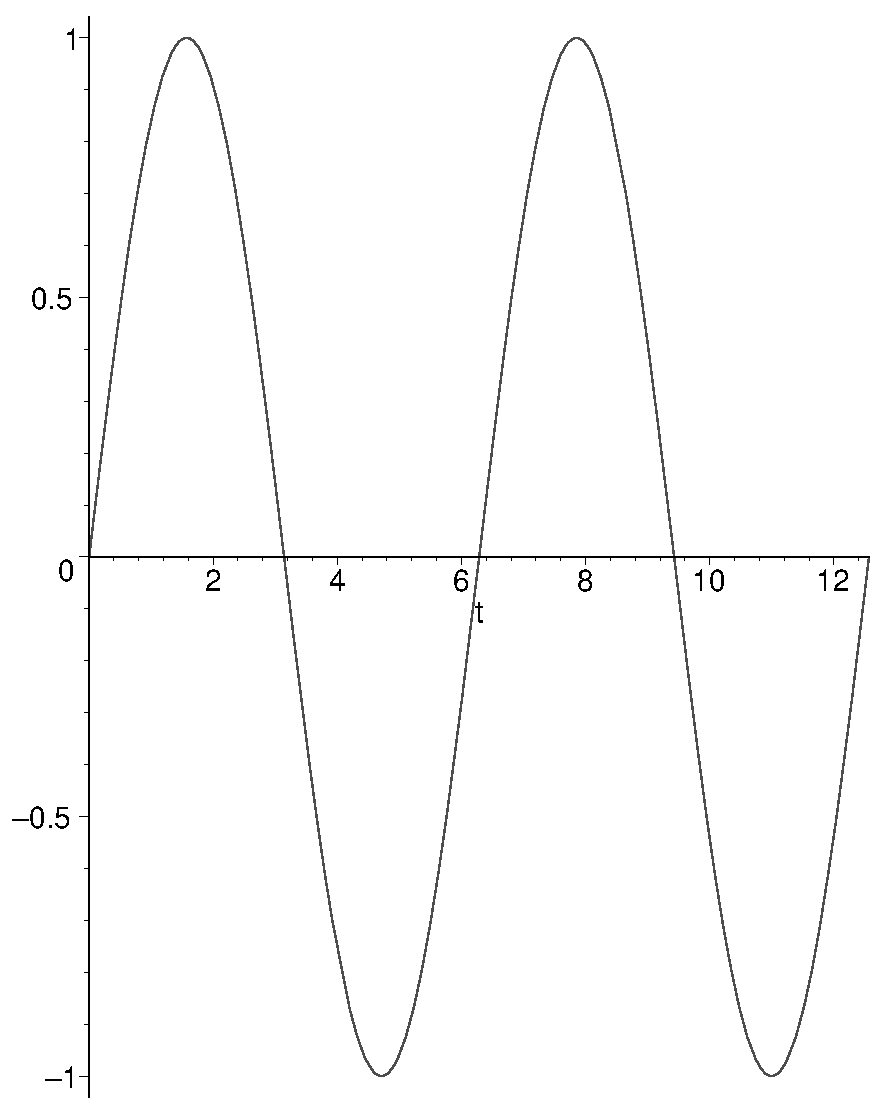
\psfig{file=sine.eps,height=3.0in}}
\caption{This here is a figure of a curve.}
\label{twodtest}
\end{figure}

